% =====================================================================
%  Introduction to Deep Learning — Class 5 (3 August)
%  Topic (course plan): Single-layer NN/Shallow NN
%  Subtopics (course plan): Regression and Classification
%  This class: the regression half.  Classification follows in Class 6.
%
%  Figures: official vector PDFs from the authors' repositories
%    - Prince figures: github.com/udlbook/udlbook (CC BY-NC-ND)
%    - Bishop figures: authors' published figure set
%  Teaching sequence for Prince figures follows his own Chapter-3
%  lecture slides (CM20315_03_Shallow).
%
%  Compile:  xelatex main.tex   (run twice)
% =====================================
%  ================================

\documentclass[aspectratio=169, 11pt]{beamer}

\usetheme{metropoliscustom}

\usepackage{graphicx}
\DeclareGraphicsExtensions{.pdf,.png,.jpg}
\graphicspath{{figs_official/}{Class05_Shallow_NN_Regression/A_Textbook_Figures/figs_official/}}
\usepackage{amsmath, amssymb}
\usepackage{bm}
\usepackage{tikz}
\usetikzlibrary{arrows.meta, positioning, calc}
\tcbuselibrary{skins}

\definecolor{mlc}{HTML}{341651}    % ML side (indigo)
\definecolor{nnc}{HTML}{800000}    % NN side (maroon)

% ---- parallel-teaching strip: split box, ML left cell / NN right cell,
%      so neither side ever wraps under the other
\newcommand{\mlparallel}[2]{%
  \vfill
  {\footnotesize
  \begin{tcolorbox}[enhanced, sidebyside, sidebyside align=top,
                    lefthand ratio=0.485,
                    segmentation style={mlc!35, line width=0.6pt},
                    colback=mlc!5, colframe=mlc!35, boxrule=0.5pt,
                    arc=1.5mm, left=2mm, right=2mm, top=0.8mm, bottom=0.8mm]
    {\color{mlc}\textbf{ML}}\;\; #1
  \tcblower
    {\color{nnc}\textbf{NN}}\;\; #2
  \end{tcolorbox}}%
  \vspace{0.6em}%
}

% ---- figure source line
\newcommand{\figsource}[1]{{\scriptsize\color{mcMuted} #1}}

% =====================================================================
\title{Single-layer NN/Shallow NN}
\subtitle{Regression and Classification}
\author{Introduction to Deep Learning \ \textperiodcentered\ Class 5
        \ \textperiodcentered\ Regression}
\institute{}
\date{3 August}

\footleft{DA3409 Introduction to Deep Learning}
\footright{Single-layer NN/Shallow NN}
\titlelogos{}

\begin{document}

\maketitle

\begin{frame}{Outline}
  \tableofcontents
\end{frame}

% =====================================================================
\section{Regression with Fixed Features}
% =====================================================================

\begin{frame}{Linear regression, two views}
  \begin{columns}[T, onlytextwidth]
    \begin{column}{0.46\textwidth}
      \centering
      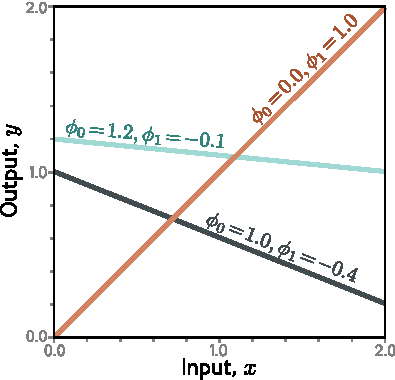
\includegraphics[height=0.44\textheight]{SupervisedLinear}
      \\[0.1em]
      \figsource{Prince (2023), Fig.~2.2.}
    \end{column}
    \hfill
    \begin{column}{0.5\textwidth}
      \vspace{0.5em}
      \[
        y = \mathrm{f}[x,\bm\phi] = \phi_0 + \phi_1 x
      \]
      \begin{itemize}\setlength{\itemsep}{1pt}
        \item Two parameters: intercept $\phi_0$,
              slope $\phi_1$
        \item Fit by minimising the \alert{least-squares
              loss}
        \item A \alert{family} of lines; parameters select
              one
      \end{itemize}
    \end{column}
  \end{columns}
  \mlparallel{model $=$ family of functions}
             {parameters select one member --- this framing
              carries through the whole course}
\end{frame}

\begin{frame}{Training: minimise the loss}
  \begin{columns}[T, onlytextwidth]
    \begin{column}{0.52\textwidth}
      \centering
      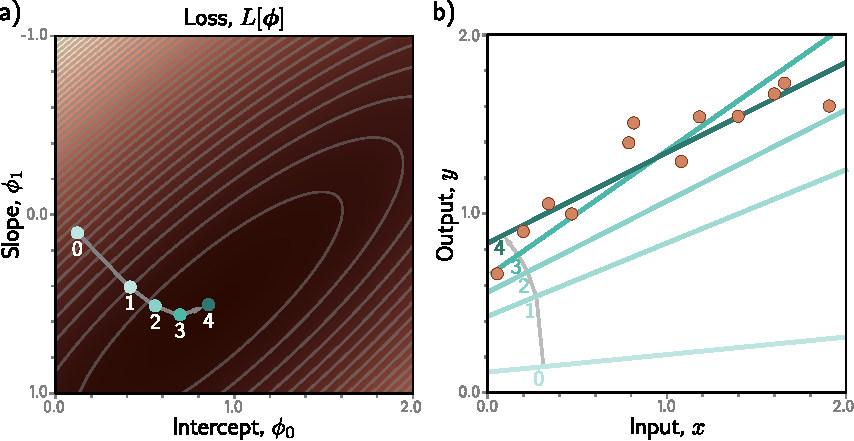
\includegraphics[width=\linewidth]{SupervisedOpt}
      \\[0.1em]
      \figsource{Prince (2023), Fig.~2.4.}
    \end{column}
    \hfill
    \begin{column}{0.44\textwidth}
      \vspace{0.3em}
      \[
        L[\bm\phi]=\sum_{i}\big(\mathrm{f}[x_i,\bm\phi]
        -y_i\big)^2
      \]
      \begin{itemize}\setlength{\itemsep}{2pt}
        \item Loss surface over $(\phi_0,\phi_1)$;
              each point is one candidate line
        \item Walk downhill: \alert{gradient descent}
        \item For a \emph{linear} model this is convex ---
              one minimum, closed form exists
      \end{itemize}
    \end{column}
  \end{columns}
\end{frame}

\begin{frame}{Beyond lines: fixed basis functions}
  Standard extension (Bishop \& Bishop, 2024, \S4.1):
  \[
    y(\mathbf{x},\mathbf{w})
    = \sum_{j=0}^{M-1} w_j\,\phi_j(\mathbf{x})
    = \mathbf{w}^{\!\top}\boldsymbol{\phi}(\mathbf{x})
    \tag{B\&B 4.3}
  \]
  \vspace{-0.2em}
  \centering
  {\small The $\phi_j$ are chosen \alert{before} seeing
  data; only $\mathbf{w}$ is learned.}
  \vspace{0.3em}
  \begin{columns}[T, onlytextwidth]
    \begin{column}{0.31\textwidth}
      \centering
      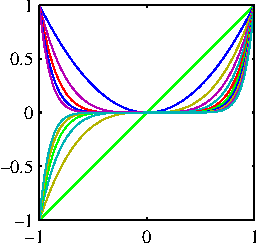
\includegraphics[height=0.27\textheight]{Bishop4_2a}\\
      \figsource{polynomials}
    \end{column}
    \begin{column}{0.31\textwidth}
      \centering
      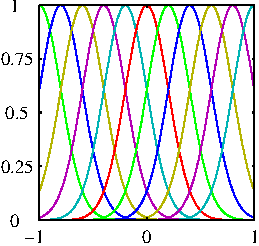
\includegraphics[height=0.27\textheight]{Bishop4_2b}\\
      \figsource{Gaussians}
    \end{column}
    \begin{column}{0.31\textwidth}
      \centering
      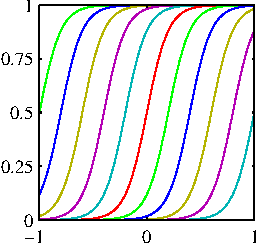
\includegraphics[height=0.27\textheight]{Bishop4_2c}\\
      \figsource{sigmoids}
    \end{column}
  \end{columns}
  \vspace{0.2em}
  \centering
  \figsource{Bishop \& Bishop (2024), Fig.~4.2.}
  \vspace{0.5em}
\end{frame}

\begin{frame}{Least squares in closed form}
  \begin{columns}[T, onlytextwidth]
    \begin{column}{0.56\textwidth}
      {\small Stack the basis functions into the
      \alert{design matrix}
      $\Phi_{nj}=\phi_j(\mathbf{x}_n)$
      (Bishop \& Bishop, 2024, Eq.~4.15). Setting
      $\nabla_{\mathbf{w}}$ of the error to zero:}
      \[
        \mathbf{w}_{\mathrm{ML}}
        = \big(\boldsymbol{\Phi}^{\!\top}\boldsymbol{\Phi}
        \big)^{-1}\boldsymbol{\Phi}^{\!\top}\mathbf{t}
        \tag{B\&B 4.14}
      \]
      \vspace{-0.6em}
      \begin{itemize}\setlength{\itemsep}{1pt}
        \item {\small The \alert{normal equations} ---
              possible because the model is
              \alert{linear in} $\mathbf{w}$}
      \end{itemize}
    \end{column}
    \hfill
    \begin{column}{0.40\textwidth}
      \centering
      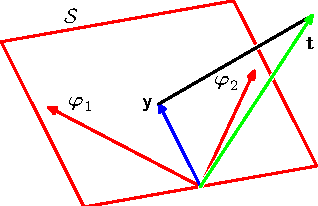
\includegraphics[width=0.74\linewidth]{Bishop4_3}
      \\[0.1em]
      \figsource{Bishop \& Bishop (2024), Fig.~4.3:
      $\boldsymbol{\Phi}\mathbf{w}_{\mathrm{ML}}$ is the
      orthogonal projection of $\mathbf{t}$.}
    \end{column}
  \end{columns}
  \mlparallel{closed form exists (Eq.~4.14)}
             {parameters inside $\mathrm{a}[\cdot]$ will
              remove the closed form}
\end{frame}

\begin{frame}{Why least squares? The probabilistic view}
  \begin{columns}[T, onlytextwidth]
    \begin{column}{0.56\textwidth}
      {\small Assume Gaussian noise around the model output
      (Bishop \& Bishop, 2024, \S4.1.1--4.1.3):}
      \[
        p(t\mid\mathbf{x},\mathbf{w},\sigma^2)
        = \mathcal{N}\big(t \mid
        y(\mathbf{x},\mathbf{w}),\,\sigma^2\big)
        \tag{B\&B 4.8}
      \]
      \vspace{-0.6em}
      \begin{itemize}\setlength{\itemsep}{1pt}
        \item {\small Max.\ log likelihood (Eq.~4.10)
              $\equiv$ min.\ \alert{sum-of-squares}
              (Eq.~4.11)}
        \item {\small Least squares $=$ \alert{maximum
              likelihood}, Gaussian noise}
      \end{itemize}
    \end{column}
    \hfill
    \begin{column}{0.40\textwidth}
      \centering
      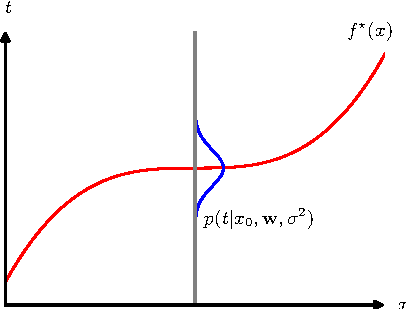
\includegraphics[width=0.66\linewidth]{Bishop4_5}
      \\[0.1em]
      \figsource{Bishop \& Bishop (2024), Fig.~4.5: the
      optimal prediction is the mean of $p(t\mid x)$.}
    \end{column}
  \end{columns}
  \mlparallel{loss $\leftarrow$ noise model: Gaussian
              $\to$ squared error}
             {Class 6 reuses this logic: Bernoulli $\to$
              cross-entropy}
\end{frame}

\begin{frame}{Linear regression is itself a network}
  \begin{columns}[T, onlytextwidth]
    \begin{column}{0.44\textwidth}
      \centering
      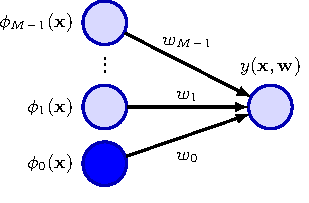
\includegraphics[width=0.7\linewidth]{Bishop4_1}
      \\[0.1em]
      \figsource{Bishop \& Bishop (2024), Fig.~4.1.}
    \end{column}
    \hfill
    \begin{column}{0.52\textwidth}
      \vspace{0.4em}
      \begin{itemize}\setlength{\itemsep}{1pt}
        \item Nodes: basis functions $\phi_j(\mathbf{x})$;
              links: weights $w_j$
        \item Already a one-layer network diagram ---
              but the $\phi_j$ \alert{carry no parameters}
      \end{itemize}
      \vspace{0.3em}
      \begin{alertblock}{The limitation}
        For images, audio, text --- nobody knows how to
        write good $\phi_j$ by hand.
      \end{alertblock}
    \end{column}
  \end{columns}
  \mlparallel{$\phi_j$ fixed by design}
             {next: make the basis functions
              \emph{adaptive}}
\end{frame}

\begin{frame}{Why shallow networks}
  A linear model in fixed features is limited. We want a model
  that is (Prince, 2023, Ch.~3 opening):
  \vspace{0.3em}
  \begin{itemize}
    \item flexible enough to describe \alert{arbitrarily
          complex} input--output mappings,
    \item able to take \alert{as many inputs} as we want,
    \item able to produce \alert{as many outputs} as we want.
  \end{itemize}
  \vspace{0.5em}
  \begin{redhighlight}
    Shallow neural networks do all three --- by putting
    parameters \emph{inside} the basis functions and learning
    them from data.
  \end{redhighlight}
\end{frame}

% =====================================================================
\section{An Example Shallow Network}
% =====================================================================

\begin{frame}{The model}
  Scalar input $x$, scalar output $y$, ten parameters
  $\bm\phi = \{\phi_0,\phi_1,\phi_2,\phi_3,\theta_{10},
  \theta_{11},\theta_{20},\theta_{21},\theta_{30},\theta_{31}\}$:
  \[
    y \;=\; \mathrm{f}[x,\bm\phi]
    \;=\; \phi_0+\phi_1\,\mathrm{a}[\theta_{10}+\theta_{11}x]
    +\phi_2\,\mathrm{a}[\theta_{20}+\theta_{21}x]
    +\phi_3\,\mathrm{a}[\theta_{30}+\theta_{31}x]
    \tag{P 3.1}
  \]
  \vspace{-0.2em}
  \begin{itemize}\setlength{\itemsep}{1pt}
    \item Represents a \alert{family of functions};
          parameters determine the particular function
    \item Given parameters: inference $=$ run the equation
    \item Given data: define a least-squares loss, change
          parameters to minimise it --- exactly as before
  \end{itemize}
  \mlparallel{$\mathbf{w}^{\!\top}\boldsymbol{\phi}(\mathbf{x})$:
              linear in fixed features}
             {Eq.~(3.1): linear in \emph{parameterised}
              features}
\end{frame}

\begin{frame}{Notation: two textbooks, same model}
  \vspace{0.15em}
  {\small
  \begin{columns}[T, onlytextwidth]
    \begin{column}{0.48\textwidth}
      \textbf{Bishop \& Bishop (2024), \S6.1}\\[0.2em]
      $a_j = \sum_{i} w_{ji}^{(1)} x_i + w_{j0}^{(1)}$
      \hfill{\scriptsize Eq.~6.1}\\[0.15em]
      $z_j = h(a_j)$
      \hfill{\scriptsize Eq.~6.2}\\[0.15em]
      $y_k = \sum_{j} w_{kj}^{(2)} z_j + w_{k0}^{(2)}$
      \hfill{\scriptsize Eq.~6.3}
    \end{column}
    \begin{column}{0.48\textwidth}
      \textbf{Prince (2023), \S3.1}\\[0.2em]
      $h_d = \mathrm{a}[\theta_{d0}+\theta_{d1}x]$
      \hfill{\scriptsize Eqs.~3.3--3.4}\\[0.15em]
      $y = \phi_0 + \sum_{d}\phi_d\,h_d$\\[0.15em]
      All parameters collectively: $\bm\phi$
    \end{column}
  \end{columns}}
  \vspace{0.3em}
  \begin{itemize}
    \item Same model: $z_j\!=\!h(a_j)$ $\equiv$
          $h_d\!=\!\mathrm{a}[\cdot]$; \;
          Bishop's $\mathbf{w}^{(2)}$ $\equiv$ Prince's
          $\phi_d$
    \item Careful: Prince's $\bm\phi$ are \alert{parameters};
          Bishop's $\boldsymbol\phi(\mathbf{x})$ are
          \alert{fixed basis functions}
    \item Equations follow Bishop where possible; Prince's
          notation accompanies his figures
  \end{itemize}
\end{frame}

\begin{frame}{The activation function: ReLU}
  \begin{columns}[T, onlytextwidth]
    \begin{column}{0.5\textwidth}
      \[
        \mathrm{a}[z]=\mathrm{ReLU}[z]=
        \begin{cases} 0 & z<0\\ z & z\ge 0\end{cases}
      \]
      \vspace{-0.3em}
      \begin{itemize}\setlength{\itemsep}{1pt}
        \item The \alert{rectified linear unit}: clips
              negative values to zero
        \item Without it, Eq.~(3.1) collapses to a single
              linear function of $x$
      \end{itemize}
    \end{column}
    \hfill
    \begin{column}{0.44\textwidth}
      \centering
      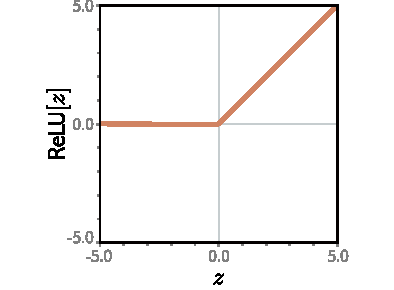
\includegraphics[height=0.40\textheight]{ShallowReLU}
      \\[0.1em]
      \figsource{Prince (2023), Fig.~3.1.}
    \end{column}
  \end{columns}
  \mlparallel{fixed nonlinearity: $x^j$, Gaussian, sigmoid}
             {nonlinearity applied to a \emph{parameterised}
              line}
\end{frame}

\begin{frame}{Hidden units: break the model into two parts}
  Stage 1 --- three linear functions, passed through the
  activation:
  \[
    h_1=\mathrm{a}[\theta_{10}+\theta_{11}x], \quad
    h_2=\mathrm{a}[\theta_{20}+\theta_{21}x], \quad
    h_3=\mathrm{a}[\theta_{30}+\theta_{31}x]
    \tag{P 3.3}
  \]
  Stage 2 --- weight and sum:
  \[
    y = \phi_0+\phi_1 h_1+\phi_2 h_2+\phi_3 h_3
    \tag{P 3.4}
  \]
  \vspace{-0.4em}
  \begin{itemize}\setlength{\itemsep}{1pt}
    \item $h_1,h_2,h_3$ are the \alert{hidden units}
          (Bishop: $z_j = h(a_j)$)
    \item Clipped $\to$ \alert{inactive}; passing its input
          $\to$ \alert{active}
  \end{itemize}
  \mlparallel{regress $y$ on fixed
              $\boldsymbol{\phi}(\mathbf{x})$}
             {Stage~2 \emph{is} linear regression --- on
              learned features $h$}
\end{frame}

\begin{frame}{Computing the function, step by step}
  \begin{columns}[T, onlytextwidth]
    \begin{column}{0.60\textwidth}
      \centering
      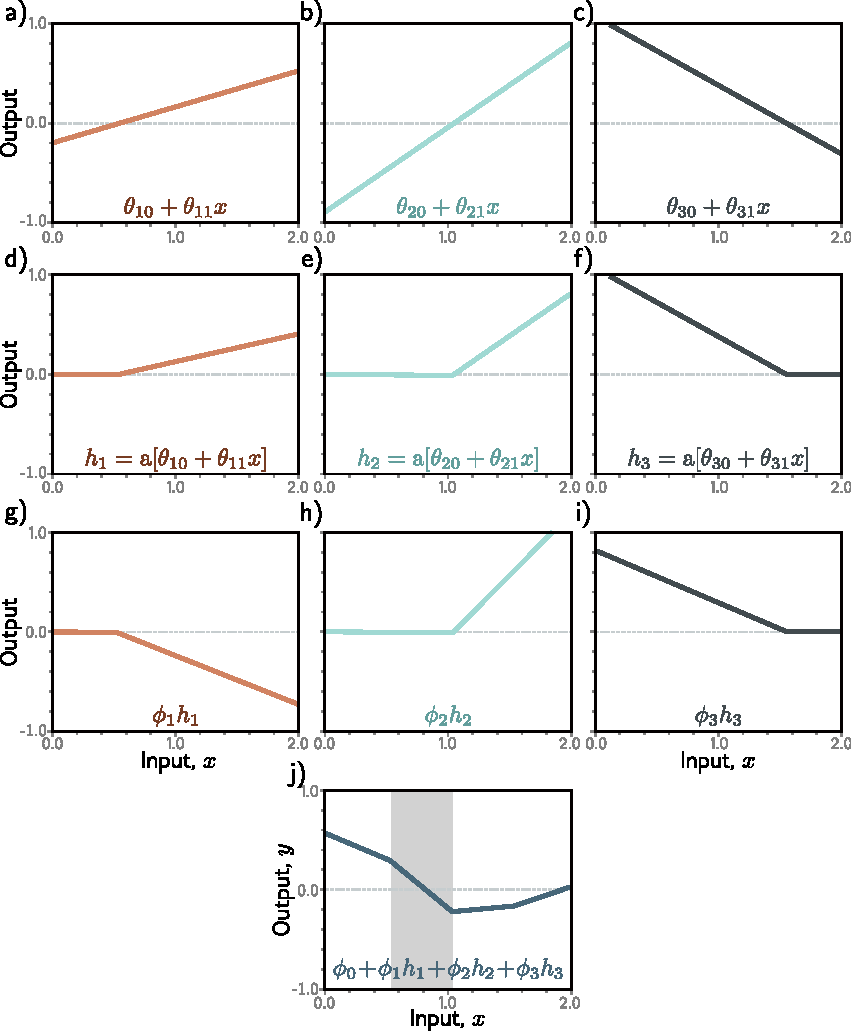
\includegraphics[height=0.74\textheight]{ShallowBuildUp}
    \end{column}
    \hfill
    \begin{column}{0.36\textwidth}
      \vspace{0.5em}
      {\small
      \begin{enumerate}\setlength{\itemsep}{4pt}
        \item[a--c)] compute three \alert{linear} functions
              $\theta_{\bullet 0}+\theta_{\bullet 1}x$
        \item[d--f)] pass each through the \alert{ReLU}
              $\to$ hidden units $h_d$
        \item[g--i)] \alert{weight} by $\phi_1,\phi_2,\phi_3$
        \item[j)] \alert{sum} plus offset $\phi_0$
      \end{enumerate}}
      \vspace{0.5em}
      \figsource{Prince (2023), Fig.~3.3;
      sequence as in his Ch.~3 lecture.}
    \end{column}
  \end{columns}
\end{frame}

\begin{frame}{The function family: piecewise linear}
  \begin{columns}[T, onlytextwidth]
    \begin{column}{0.58\textwidth}
      \centering
      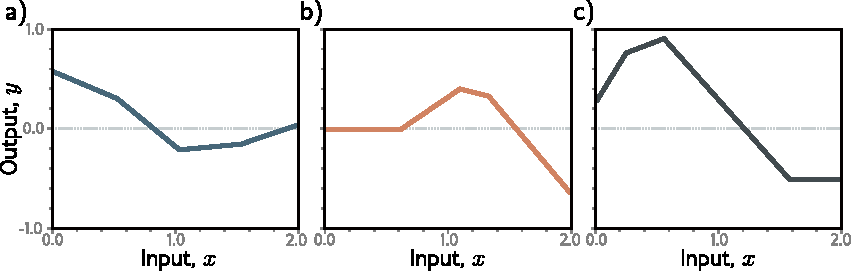
\includegraphics[width=0.88\linewidth]{ShallowFunctions}
      \\[0.1em]
      \figsource{Prince (2023), Fig.~3.2.}
    \end{column}
    \hfill
    \begin{column}{0.38\textwidth}
      \vspace{0.3em}
      \begin{itemize}\setlength{\itemsep}{2pt}
        \item Continuous piecewise-linear functions
        \item One \alert{``joint'' per ReLU}: three
              units $\to$ up to four regions
        \item Each region $\leftrightarrow$ an
              \alert{activation pattern}: which units
              are active
      \end{itemize}
    \end{column}
  \end{columns}
  \mlparallel{family: span of chosen basis functions}
             {family: piecewise-linear, joints placed by
              training}
\end{frame}

\begin{frame}{Depicting the network}
  \centering
  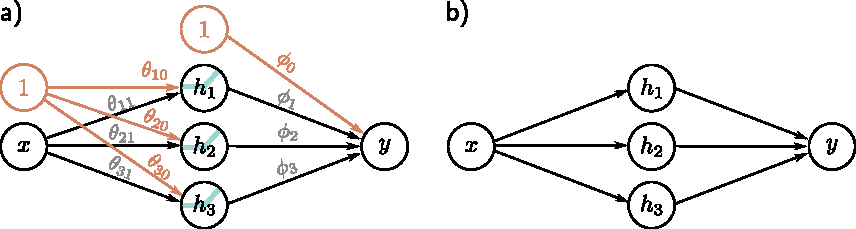
\includegraphics[width=0.62\linewidth]{ShallowNet}
  \\[0.15em]
  \figsource{Prince (2023), Fig.~3.4.}
  \vspace{0.3em}
  \begin{itemize}
    \item Each \alert{parameter multiplies its source and
          adds to its target}
    \item (b) is the standard shorthand: intercepts
          (offsets) usually not drawn
  \end{itemize}
\end{frame}

\begin{frame}{Bishop's picture: learned basis functions}
  \begin{columns}[T, onlytextwidth]
    \begin{column}{0.23\textwidth}
      \centering
      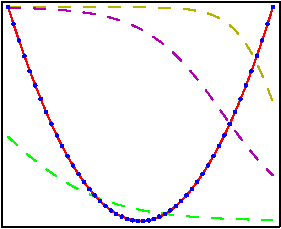
\includegraphics[width=\linewidth]{Bishop6_10a}
    \end{column}
    \begin{column}{0.23\textwidth}
      \centering
      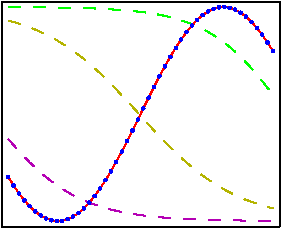
\includegraphics[width=\linewidth]{Bishop6_10b}
    \end{column}
    \begin{column}{0.23\textwidth}
      \centering
      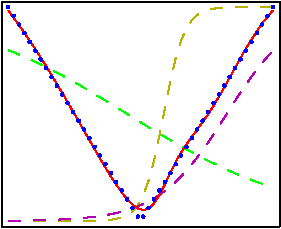
\includegraphics[width=\linewidth]{Bishop6_10c}
    \end{column}
    \begin{column}{0.23\textwidth}
      \centering
      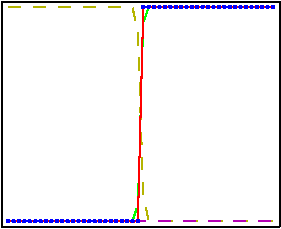
\includegraphics[width=\linewidth]{Bishop6_10d}
    \end{column}
  \end{columns}
  \vspace{0.2em}
  \centering
  \figsource{Bishop \& Bishop (2024), Fig.~6.10: dashed
  curves $=$ hidden units $z_j$ ($\tanh$); red curve $=$
  network output.}
  \vspace{0.4em}
  \begin{itemize}
    \item Same architecture, $\tanh$ activation: hidden
          units act as \alert{basis functions that adapt}
          to each dataset
    \item Four different target functions --- the same
          network learns four different bases
  \end{itemize}
\end{frame}

% =====================================================================
\section{Generalising the Network}
% =====================================================================

\begin{frame}{Capacity: $D$ hidden units}
  \[
    h_d=\mathrm{a}[\theta_{d0}+\theta_{d1}x],
    \qquad
    y=\phi_0+\sum_{d=1}^{D}\phi_d h_d
    \tag{P 3.5--3.6}
  \]
  \begin{itemize}
    \item The number of hidden units $D$ is a measure of
          \alert{network capacity}
    \item $D$ ReLU units: $D$ joints $\to$ at most
          \alert{$D{+}1$ linear regions}
  \end{itemize}
  \mlparallel{capacity dial: polynomial degree / \#basis
              functions $M$}
             {capacity dial: hidden units $D$}
\end{frame}

\begin{frame}{Universal approximation}
  \begin{columns}[T, onlytextwidth]
    \begin{column}{0.58\textwidth}
      \centering
      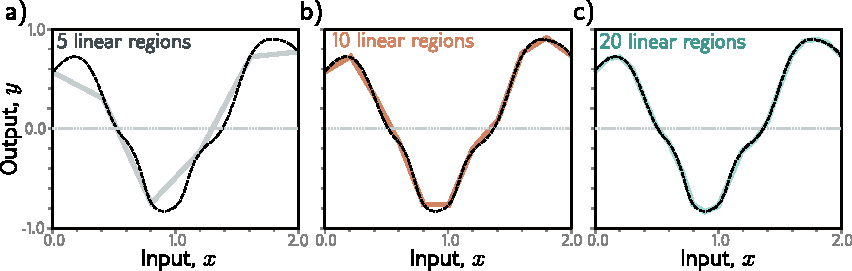
\includegraphics[width=0.86\linewidth]{ShallowApproximate}
      \\[0.1em]
      \figsource{Prince (2023), Fig.~3.5.}
    \end{column}
    \hfill
    \begin{column}{0.38\textwidth}
      {\small
      With enough hidden units, a shallow network can
      describe \alert{any continuous function} to arbitrary
      precision --- the \alert{universal approximation
      theorem} (Prince, 2023, \S3.2).}
      \vspace{0.3em}
      \begin{itemize}\setlength{\itemsep}{1pt}
        \item {\small One more region per unit; more
              regions $\to$ closer fit}
        \item {\small Existence --- not a construction, not a
              size bound (Cybenko 1989; Hornik 1991)}
      \end{itemize}
    \end{column}
  \end{columns}
\end{frame}

\begin{frame}{More than one output}
  \begin{columns}[T, onlytextwidth]
    \begin{column}{0.60\textwidth}
      \centering
      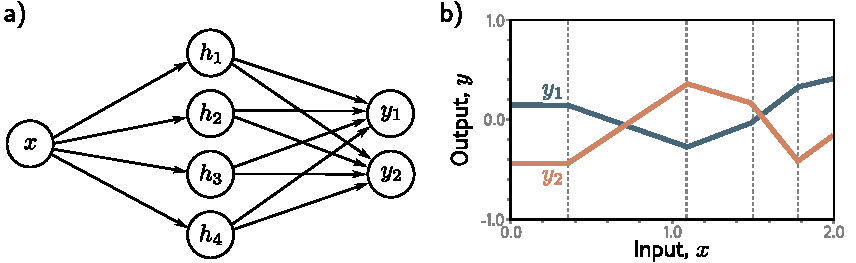
\includegraphics[width=\linewidth]{ShallowNetTwoOutputs}
      \\[0.1em]
      \figsource{Prince (2023), Fig.~3.6.}
    \end{column}
    \hfill
    \begin{column}{0.36\textwidth}
      \vspace{0.3em}
      {\small 1 input, 4 hidden units, 2 outputs:}
      \[
        y_k=\phi_{k0}+\textstyle\sum_{d}\phi_{kd}h_d
      \]
      \begin{itemize}\setlength{\itemsep}{2pt}
        \item {\small One extra linear read-out per output
              --- hidden units are \alert{shared}}
        \item {\small Hence both outputs have joints at
              the \alert{same places}}
      \end{itemize}
    \end{column}
  \end{columns}
\end{frame}

\begin{frame}{More than one input}
  \begin{columns}[T, onlytextwidth]
    \begin{column}{0.55\textwidth}
      \centering
      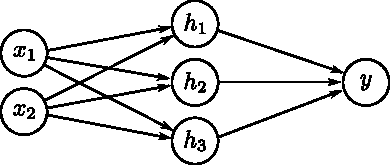
\includegraphics[width=\linewidth]{ShallowNetTwoInputs}
      \\[0.1em]
      \figsource{Prince (2023), Fig.~3.7.}
    \end{column}
    \hfill
    \begin{column}{0.41\textwidth}
      \vspace{0.3em}
      {\small 2 inputs, 3 hidden units, 1 output:}
      \[
        h_d=\mathrm{a}[\theta_{d0}+\theta_{d1}x_1
        +\theta_{d2}x_2]
      \]
      \begin{itemize}\setlength{\itemsep}{2pt}
        \item {\small One slope per input: each
              pre-activation is an \alert{oriented plane}
              over the input space}
      \end{itemize}
    \end{column}
  \end{columns}
\end{frame}

\begin{frame}{Two inputs, computed step by step}
  \begin{columns}[T, onlytextwidth]
    \begin{column}{0.56\textwidth}
      \centering
      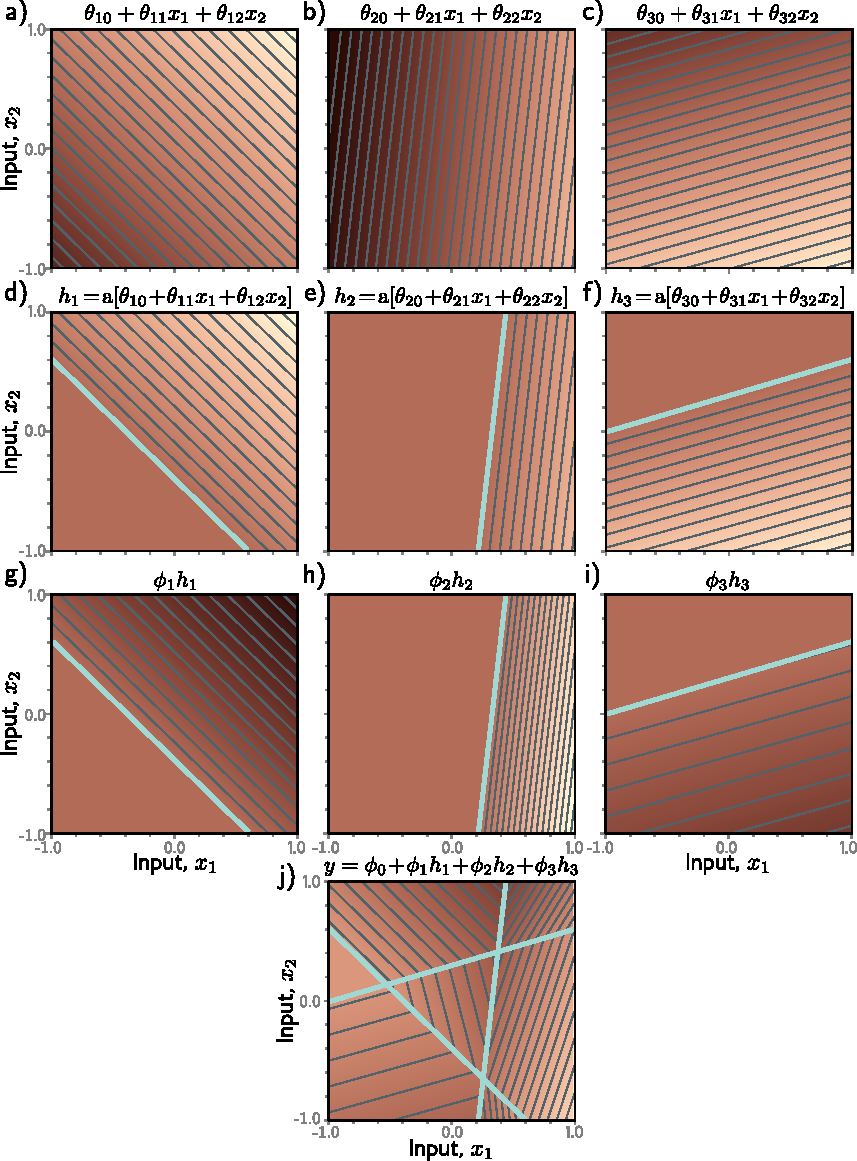
\includegraphics[height=0.76\textheight]{ShallowBuildUp2D}
    \end{column}
    \hfill
    \begin{column}{0.40\textwidth}
      \vspace{0.5em}
      {\small
      \begin{enumerate}\setlength{\itemsep}{4pt}
        \item[a--c)] three linear functions
              (\alert{oriented planes}) of $x_1,x_2$
        \item[d--f)] clipped by ReLU $\to$ hidden units
        \item[g--i)] weighted by $\phi_d$
        \item[j)] summed $+$ offset
      \end{enumerate}
      \vspace{0.3em}
      The linear regions are \alert{convex polygons}, one
      per activation pattern.}
      \vspace{0.4em}
      \figsource{Prince (2023), Fig.~3.8.}
    \end{column}
  \end{columns}
\end{frame}

\begin{frame}{The general case}
  \begin{columns}[T, onlytextwidth]
    \begin{column}{0.45\textwidth}
      \centering
      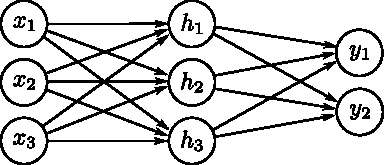
\includegraphics[width=0.9\linewidth]{ShallowNetThreeInputsTwoOutputs}
      \\[0.1em]
      \figsource{Prince (2023), Fig.~3.12.}
    \end{column}
    \hfill
    \begin{column}{0.51\textwidth}
      \vspace{0.2em}
      {\small $D_i$ inputs, $D$ hidden units, $D_o$
      outputs (Bishop notation, Eqs.~6.1--6.3):}
      \[
        z_j = h\Big(\textstyle\sum_i w_{ji}^{(1)}x_i
        + w_{j0}^{(1)}\Big)
      \]
      \[
        y_k = \textstyle\sum_j w_{kj}^{(2)}z_j
        + w_{k0}^{(2)}
      \]
      \begin{itemize}\setlength{\itemsep}{2pt}
        \item {\small e.g.\ three inputs, three hidden
              units, two outputs $\to$ 20 parameters}
      \end{itemize}
    \end{column}
  \end{columns}
\end{frame}

\begin{frame}{The same picture in Bishop's notation}
  \begin{columns}[T, onlytextwidth]
    \begin{column}{0.52\textwidth}
      \centering
      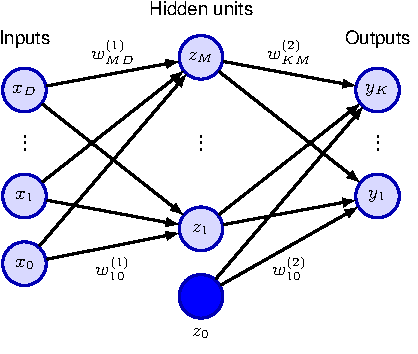
\includegraphics[width=0.95\linewidth]{Bishop6_9}
      \\[0.1em]
      \figsource{Bishop \& Bishop (2024), Fig.~6.9.}
    \end{column}
    \hfill
    \begin{column}{0.44\textwidth}
      \vspace{0.3em}
      \begin{itemize}\setlength{\itemsep}{3pt}
        \item Weights carry \alert{layer superscripts}:
              $w^{(1)}_{ji}$ into the hidden layer,
              $w^{(2)}_{kj}$ out of it
        \item Biases drawn as links from clamped units
              $x_0\!=\!1$, $z_0\!=\!1$
        \item $D$ inputs, $M$ hidden units, $K$ outputs
              --- exactly Eqs.~(6.1)--(6.3)
      \end{itemize}
    \end{column}
  \end{columns}
\end{frame}

\begin{frame}{How many regions?}
  \begin{columns}[T, onlytextwidth]
    \begin{column}{0.40\textwidth}
      \centering
      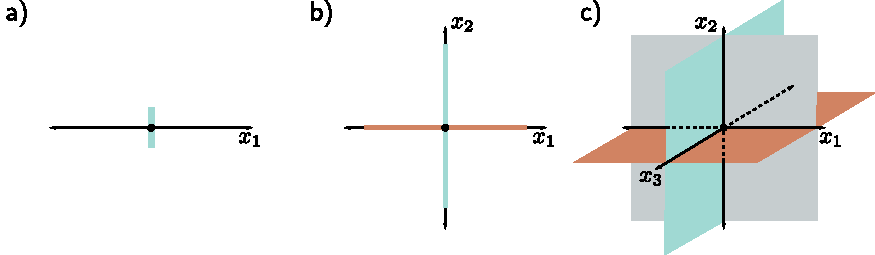
\includegraphics[width=\linewidth]{ShallowHyperplanes}
      \\[0.1em]
      \figsource{Prince (2023), Fig.~3.10: each hidden unit
      is a hyperplane cutting input space.}
    \end{column}
    \hfill
    \begin{column}{0.54\textwidth}
      \centering
      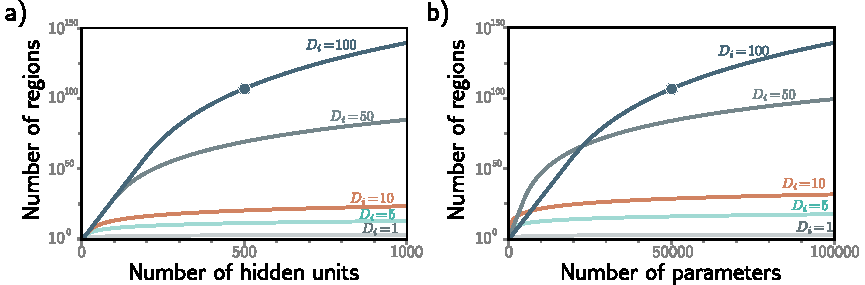
\includegraphics[width=\linewidth]{ShallowRegions}
      \\[0.1em]
      \figsource{Prince (2023), Fig.~3.9.}
    \end{column}
  \end{columns}
  \vspace{0.3em}
  \begin{itemize}
    \item Zaslavsky (1975): $D$ hyperplanes in
          $D_i$-dimensional input space create at most
          $\sum_{j=0}^{D_i}\binom{D}{j}$ regions ---
          \alert{binomial coefficients}
    \item Highlighted point: $D\!=\!500$ units
          ($51{,}001$ parameters) $\to$ more than
          $10^{107}$ regions
  \end{itemize}
\end{frame}

\begin{frame}{Terminology}
  \begin{columns}[T, onlytextwidth]
    \begin{column}{0.52\textwidth}
      \centering
      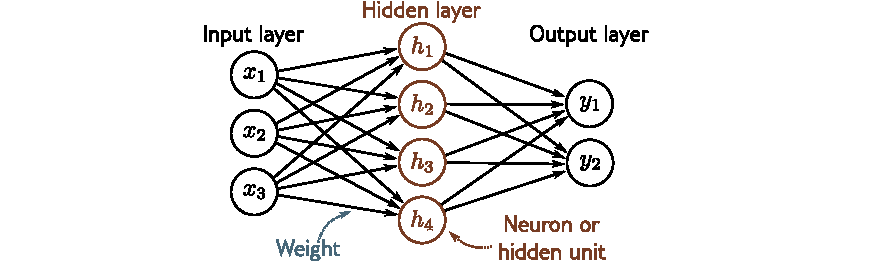
\includegraphics[width=\linewidth]{ShallowTerminology}
      \\[0.1em]
      \figsource{Prince (2023), Fig.~3.11.}
    \end{column}
    \hfill
    \begin{column}{0.44\textwidth}
      \vspace{0.3em}
      \begin{itemize}\setlength{\itemsep}{2pt}
        \item \alert{input layer} / \alert{hidden layer} /
              \alert{output layer}
        \item weights (slopes) and \alert{biases}
              (offsets)
        \item pre-activations $a_j$, activations
              $z_j$
        \item \alert{fully connected, feed-forward};
          one hidden layer $=$ \alert{shallow}
        \item with $\ge 1$ hidden layer, also called a
              \alert{multi-layer perceptron}
      \end{itemize}
    \end{column}
  \end{columns}
\end{frame}

\begin{frame}{Other activation functions}
  \centering
  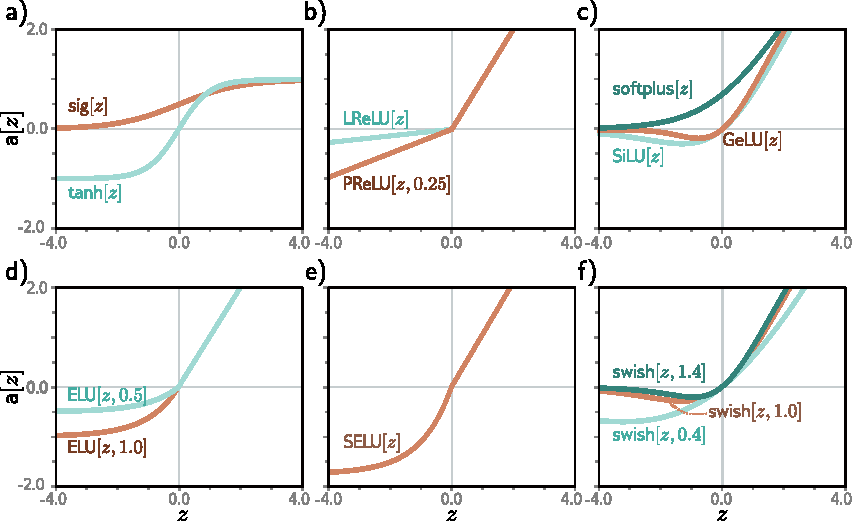
\includegraphics[height=0.58\textheight]{ShallowActivations}
  \\[0.1em]
  \figsource{Prince (2023), Fig.~3.13: sigmoid, tanh,
  leaky ReLU, GeLU, SiLU, ELU, and others. ReLU is the
  modern default; tanh/sigmoid were historically standard.}
\end{frame}

\begin{frame}{Bishop's gallery of activations}
  \begin{columns}[T, onlytextwidth]
    \begin{column}{0.31\textwidth}
      \centering
      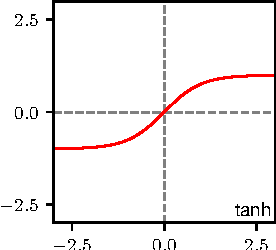
\includegraphics[width=0.7\linewidth]{Bishop6_12a}
    \end{column}
    \begin{column}{0.31\textwidth}
      \centering
      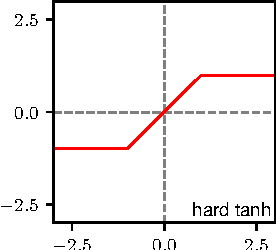
\includegraphics[width=0.7\linewidth]{Bishop6_12b}
    \end{column}
    \begin{column}{0.31\textwidth}
      \centering
      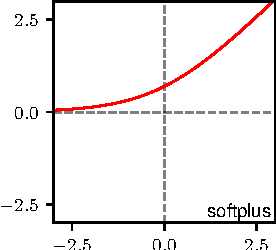
\includegraphics[width=0.7\linewidth]{Bishop6_12c}
    \end{column}
  \end{columns}
  \vspace{0.3em}
  \begin{columns}[T, onlytextwidth]
    \begin{column}{0.31\textwidth}
      \centering
      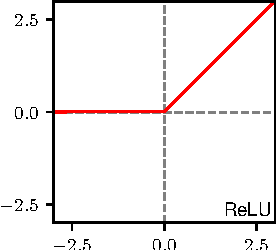
\includegraphics[width=0.7\linewidth]{Bishop6_12d}
    \end{column}
    \begin{column}{0.31\textwidth}
      \centering
      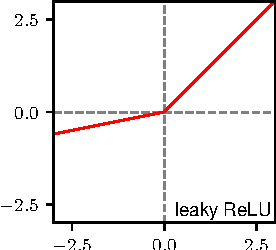
\includegraphics[width=0.7\linewidth]{Bishop6_12e}
    \end{column}
    \begin{column}{0.31\textwidth}
      \centering
      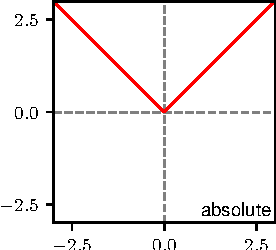
\includegraphics[width=0.7\linewidth]{Bishop6_12f}
    \end{column}
  \end{columns}
  \vspace{0.2em}
  \centering
  \figsource{Bishop \& Bishop (2024), Fig.~6.12: tanh,
  hard tanh, softplus, ReLU, leaky ReLU, absolute.}
\end{frame}

% =====================================================================
\section{Training}
% =====================================================================

\begin{frame}{Same loss, harder landscape}
  Sum-of-squares error, now with a network inside
  (Bishop \& Bishop, 2024, \S6.1):
  \[
    E(\mathbf{w}) = \tfrac{1}{2}\textstyle\sum_{n}
    \lVert \mathbf{y}(\mathbf{x}_n,\mathbf{w})
    - \mathbf{t}_n\rVert^2
  \]
  \vspace{-0.3em}
  \begin{itemize}\setlength{\itemsep}{1pt}
    \item Parameters sit inside $h(\cdot)$:
          $\nabla E = \mathbf{0}$ has \alert{no closed
          form}
    \item The loss surface is \alert{non-convex} ---
          unlike every model so far
    \item Training: gradient descent, as on the
          Fig.~2.4 surface --- Classes 11--13
  \end{itemize}
  \mlparallel{normal equations: jump to the minimum,
              convex}
             {gradient descent: walk downhill, non-convex}
\end{frame}

\begin{frame}{Weight-space symmetries}
  The non-convexity is \alert{structural}
  (Bishop \& Bishop, 2024, \S6.1.1):
  \vspace{0.2em}
  \begin{itemize}
    \item \alert{Sign-flip}: flipping the sign of all
          weights into and out of a hidden unit gives the
          same function
    \item \alert{Permutation}: relabelling hidden units
          gives the same function --- $M!$ equivalent
          weight vectors
    \item Every minimum appears at least $M!\cdot 2^M$
          times in weight space --- the same function,
          many addresses
  \end{itemize}
\end{frame}

\begin{frame}{It works: shallow networks fit real data}
  \begin{columns}[T, onlytextwidth]
    \begin{column}{0.47\textwidth}
      \centering
      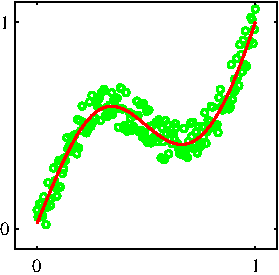
\includegraphics[height=0.52\textheight]{Bishop6_17a}
    \end{column}
    \hfill
    \begin{column}{0.47\textwidth}
      \centering
      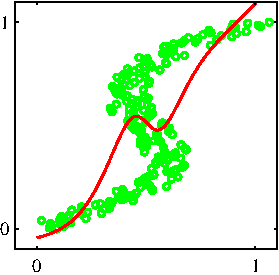
\includegraphics[height=0.52\textheight]{Bishop6_17b}
    \end{column}
  \end{columns}
  \vspace{0.2em}
  \centering
  \figsource{Bishop \& Bishop (2024), Fig.~6.17: two-layer
  network fits (red) to noisy data (green). Trained by
  gradient descent on the sum-of-squares error; the learned
  hidden units place their joints where the data demands.}
\end{frame}

\begin{frame}{The dictionary}
  \centering
  \renewcommand{\arraystretch}{1.12}
  {\footnotesize
  \begin{tabular}{p{0.20\textwidth} p{0.35\textwidth}
                  p{0.35\textwidth}}
    & \textbf{\color{mlc}Linear/Basis-Function Model}
    & \textbf{\color{nnc}Shallow Neural Network}\\
    \hline
    Function class
      & lines, polynomials, RBFs
      & piecewise-linear surfaces\\
    Features
      & $\phi_j(\mathbf{x})$, fixed
      & $z_j=h(a_j)$, learned\\
    Prediction
      & $\mathbf{w}^{\!\top}\boldsymbol{\phi}(\mathbf{x})$
      & $\sum_j w_{kj}^{(2)} z_j + w_{k0}^{(2)}$\\
    Loss (regression)
      & sum of squares
      & sum of squares\\
    Optimisation
      & normal equations, convex
      & gradient descent, non-convex\\
    Capacity
      & \#basis functions $M$
      & hidden units $D$, regions
        $\le\sum_j\binom{D}{j}$\\
    \hline
  \end{tabular}}
  \vspace{0.5em}
  \begin{redhighlight}
    A shallow network is regression whose basis functions
    carry parameters and are learned from data.
  \end{redhighlight}
\end{frame}

\begin{frame}{Takeaways}
  \begin{enumerate}
    \item A shallow network puts parameters inside the
          basis functions; the output layer is a
          \alert{linear regression on learned features}
    \item With ReLU the family is \alert{piecewise
          linear}: one joint per unit, regions counted by
          binomial coefficients
    \item With enough units it approximates \alert{any
          continuous function} --- existence, not a
          construction
    \item The price: \alert{no closed form}, a non-convex
          loss, and gradient-based training
  \end{enumerate}
  \vspace{0.4em}
  \begin{redhighlight}
    Class~6: the same architecture for
    \alert{classification} --- sigmoid/softmax outputs and
    cross-entropy loss.
  \end{redhighlight}
\end{frame}

\begin{frame}{References}
  \footnotesize
  \begin{itemize}
    \item C.~M.~Bishop \& H.~Bishop. \textit{Deep
          Learning: Foundations and Concepts.} Springer,
          2024. \S4.1, \S6.1. Figures 4.1, 4.2, 6.10,
          6.17 from the authors' published figure set,
          with attribution.
    \item S.~J.~D.~Prince. \textit{Understanding Deep
          Learning.} MIT Press, 2023. Ch.~2--3. Figures
          2.2, 2.4, 3.1--3.13 and teaching sequence from
          the author's repository
          (\url{https://udlbook.github.io/udlbook/}),
          CC BY-NC-ND, with attribution.
    \item G.~Cybenko (1989); K.~Hornik (1991);
          T.~Zaslavsky (1975).
  \end{itemize}
\end{frame}

\begin{frame}[standout]
  Questions?
\end{frame}

\end{document}
